\documentclass[11pt,a4paper]{article}
\usepackage[margin=2.3cm]{geometry}
\usepackage[T1]{fontenc}
\usepackage{mathptmx}
\usepackage{amsmath,amssymb}
\usepackage{booktabs,array,graphicx,caption,subcaption}
\usepackage{algorithm}
\usepackage{algpseudocode}
\usepackage[numbers,sort&compress]{natbib}
\usepackage[hidelinks]{hyperref}
\usepackage{lineno}
\newcommand{\NRec}{374}
\newcommand{\NUnique}{132}
\newcommand{\NVec}{109}
\newcommand{\NDup}{242}
\newcommand{\NConflictVec}{22}
\newcommand{\NConflictRows}{128}
\newcommand{\NNone}{219}
\newcommand{\NIns}{77}
\newcommand{\NApn}{78}
\newcommand{\NUniqNone}{73}
\newcommand{\NUniqIns}{29}
\newcommand{\NUniqApn}{30}
\newcommand{\OrigLeak}{68}
\newcommand{\OrigNovel}{7}
\newcommand{\OrigSameLabel}{65}
\newcommand{\Ceiling}{93.3}
\newcommand{\CeilingRows}{349}
\newcommand{\TrainAccRF}{93.0}
\newcommand{\TrainAccStack}{93.0}
\newcommand{\TrainAccXGB}{92.8}
\newcommand{\OrigStackCorrect}{72}
\newcommand{\OrigStackAcc}{96.00}
\newcommand{\OrigStackCPlo}{88.8}
\newcommand{\OrigStackCPhi}{99.2}
\newcommand{\OrigStackF}{0.94}
\newcommand{\OrigStackTrain}{91.6}
\newcommand{\OrigStackNovelAcc}{71.4}
\newcommand{\OrigStackNovelCorrect}{5}
\newcommand{\OrigVoteCorrect}{72}
\newcommand{\OrigVoteAcc}{96.00}
\newcommand{\OrigVoteCPlo}{88.8}
\newcommand{\OrigVoteCPhi}{99.2}
\newcommand{\OrigVoteF}{0.94}
\newcommand{\OrigVoteTrain}{91.6}
\newcommand{\OrigVoteNovelAcc}{85.7}
\newcommand{\OrigVoteNovelCorrect}{6}
\newcommand{\OrigRFCorrect}{72}
\newcommand{\OrigRFAcc}{96.00}
\newcommand{\OrigRFCPlo}{88.8}
\newcommand{\OrigRFCPhi}{99.2}
\newcommand{\OrigRFF}{0.94}
\newcommand{\OrigRFTrain}{92.0}
\newcommand{\OrigRFNovelAcc}{85.7}
\newcommand{\OrigRFNovelCorrect}{6}
\newcommand{\OrigXGBCorrect}{70}
\newcommand{\OrigXGBAcc}{93.33}
\newcommand{\OrigXGBCPlo}{85.1}
\newcommand{\OrigXGBCPhi}{97.8}
\newcommand{\OrigXGBF}{0.89}
\newcommand{\OrigXGBTrain}{91.6}
\newcommand{\OrigXGBNovelAcc}{57.1}
\newcommand{\OrigXGBNovelCorrect}{4}
\newcommand{\OrigLRCorrect}{71}
\newcommand{\OrigLRAcc}{94.67}
\newcommand{\OrigLRCPlo}{86.9}
\newcommand{\OrigLRCPhi}{98.5}
\newcommand{\OrigLRF}{0.92}
\newcommand{\OrigLRTrain}{91.0}
\newcommand{\OrigLRNovelAcc}{85.7}
\newcommand{\OrigLRNovelCorrect}{6}
\newcommand{\OrigStackOnly}{1}
\newcommand{\OrigVoteOnly}{1}
\newcommand{\OrigMcnemar}{1.00}
\newcommand{\OrigBootLo}{-4.0}
\newcommand{\OrigBootHi}{4.0}
\newcommand{\OrigMDE}{5.3}
\newcommand{\AccStackG}{89.6}
\newcommand{\FStackG}{0.87}
\newcommand{\BrierStackG}{0.186}
\newcommand{\AucStackG}{0.91}
\newcommand{\CIloStackG}{86.1}
\newcommand{\CIhiStackG}{92.7}
\newcommand{\FoldSDStackG}{3.8}
\newcommand{\RepSDStackG}{0.53}
\newcommand{\EceStackG}{0.062}
\newcommand{\LlStackG}{0.446}
\newcommand{\AccVoteG}{89.8}
\newcommand{\FVoteG}{0.87}
\newcommand{\BrierVoteG}{0.184}
\newcommand{\AucVoteG}{0.92}
\newcommand{\CIloVoteG}{86.3}
\newcommand{\CIhiVoteG}{92.9}
\newcommand{\FoldSDVoteG}{3.6}
\newcommand{\RepSDVoteG}{0.60}
\newcommand{\EceVoteG}{0.060}
\newcommand{\LlVoteG}{0.447}
\newcommand{\AccLRG}{89.7}
\newcommand{\FLRG}{0.87}
\newcommand{\BrierLRG}{0.188}
\newcommand{\AucLRG}{0.92}
\newcommand{\CIloLRG}{86.0}
\newcommand{\CIhiLRG}{92.8}
\newcommand{\FoldSDLRG}{4.0}
\newcommand{\RepSDLRG}{0.35}
\newcommand{\EceLRG}{0.063}
\newcommand{\LlLRG}{0.435}
\newcommand{\AccRFG}{89.8}
\newcommand{\FRFG}{0.87}
\newcommand{\BrierRFG}{0.191}
\newcommand{\AucRFG}{0.92}
\newcommand{\CIloRFG}{86.4}
\newcommand{\CIhiRFG}{92.9}
\newcommand{\FoldSDRFG}{3.7}
\newcommand{\RepSDRFG}{0.58}
\newcommand{\EceRFG}{0.079}
\newcommand{\LlRFG}{1.119}
\newcommand{\AccXGBG}{89.8}
\newcommand{\FXGBG}{0.87}
\newcommand{\BrierXGBG}{0.185}
\newcommand{\AucXGBG}{0.92}
\newcommand{\CIloXGBG}{86.3}
\newcommand{\CIhiXGBG}{92.9}
\newcommand{\FoldSDXGBG}{3.6}
\newcommand{\RepSDXGBG}{0.75}
\newcommand{\EceXGBG}{0.055}
\newcommand{\LlXGBG}{0.431}
\newcommand{\AccMajG}{58.6}
\newcommand{\FMajG}{0.25}
\newcommand{\BrierMajG}{0.571}
\newcommand{\AucMajG}{0.50}
\newcommand{\CIloMajG}{47.6}
\newcommand{\CIhiMajG}{68.6}
\newcommand{\FoldSDMajG}{0.7}
\newcommand{\RepSDMajG}{0.00}
\newcommand{\EceMajG}{0.006}
\newcommand{\LlMajG}{0.966}
\newcommand{\AccTreeG}{88.1}
\newcommand{\FTreeG}{0.85}
\newcommand{\BrierTreeG}{0.209}
\newcommand{\AucTreeG}{0.90}
\newcommand{\CIloTreeG}{84.1}
\newcommand{\CIhiTreeG}{91.4}
\newcommand{\FoldSDTreeG}{4.3}
\newcommand{\RepSDTreeG}{0.46}
\newcommand{\EceTreeG}{0.044}
\newcommand{\LlTreeG}{0.775}
\newcommand{\AccSVMG}{90.0}
\newcommand{\FSVMG}{0.87}
\newcommand{\BrierSVMG}{0.172}
\newcommand{\AucSVMG}{0.93}
\newcommand{\CIloSVMG}{86.7}
\newcommand{\CIhiSVMG}{92.9}
\newcommand{\FoldSDSVMG}{4.0}
\newcommand{\RepSDSVMG}{0.87}
\newcommand{\EceSVMG}{0.027}
\newcommand{\LlSVMG}{0.369}
\newcommand{\AccCatG}{89.8}
\newcommand{\FCatG}{0.87}
\newcommand{\BrierCatG}{0.180}
\newcommand{\AucCatG}{0.92}
\newcommand{\CIloCatG}{86.3}
\newcommand{\CIhiCatG}{92.7}
\newcommand{\FoldSDCatG}{4.0}
\newcommand{\RepSDCatG}{0.61}
\newcommand{\EceCatG}{0.045}
\newcommand{\LlCatG}{0.397}
\newcommand{\AccStackD}{73.0}
\newcommand{\FStackD}{0.67}
\newcommand{\BrierStackD}{0.452}
\newcommand{\AucStackD}{0.77}
\newcommand{\CIloStackD}{66.9}
\newcommand{\CIhiStackD}{79.0}
\newcommand{\FoldSDStackD}{8.5}
\newcommand{\RepSDStackD}{2.41}
\newcommand{\EceStackD}{0.126}
\newcommand{\LlStackD}{0.900}
\newcommand{\AccVoteD}{72.2}
\newcommand{\FVoteD}{0.65}
\newcommand{\BrierVoteD}{0.478}
\newcommand{\AucVoteD}{0.75}
\newcommand{\CIloVoteD}{65.2}
\newcommand{\CIhiVoteD}{79.6}
\newcommand{\FoldSDVoteD}{7.9}
\newcommand{\RepSDVoteD}{1.79}
\newcommand{\EceVoteD}{0.148}
\newcommand{\LlVoteD}{0.977}
\newcommand{\AccLRD}{74.1}
\newcommand{\FLRD}{0.68}
\newcommand{\BrierLRD}{0.435}
\newcommand{\AucLRD}{0.78}
\newcommand{\CIloLRD}{68.3}
\newcommand{\CIhiLRD}{80.0}
\newcommand{\FoldSDLRD}{7.9}
\newcommand{\RepSDLRD}{1.79}
\newcommand{\EceLRD}{0.121}
\newcommand{\LlLRD}{0.838}
\newcommand{\AccRFD}{73.4}
\newcommand{\FRFD}{0.66}
\newcommand{\BrierRFD}{0.482}
\newcommand{\AucRFD}{0.75}
\newcommand{\CIloRFD}{66.6}
\newcommand{\CIhiRFD}{80.5}
\newcommand{\FoldSDRFD}{6.9}
\newcommand{\RepSDRFD}{1.64}
\newcommand{\EceRFD}{0.149}
\newcommand{\LlRFD}{1.885}
\newcommand{\AccXGBD}{70.9}
\newcommand{\FXGBD}{0.64}
\newcommand{\BrierXGBD}{0.486}
\newcommand{\AucXGBD}{0.75}
\newcommand{\CIloXGBD}{63.8}
\newcommand{\CIhiXGBD}{78.5}
\newcommand{\FoldSDXGBD}{8.0}
\newcommand{\RepSDXGBD}{2.47}
\newcommand{\EceXGBD}{0.145}
\newcommand{\LlXGBD}{0.941}
\newcommand{\AccMajD}{55.3}
\newcommand{\FMajD}{0.24}
\newcommand{\BrierMajD}{0.594}
\newcommand{\AucMajD}{0.50}
\newcommand{\CIloMajD}{47.7}
\newcommand{\CIhiMajD}{63.4}
\newcommand{\FoldSDMajD}{1.4}
\newcommand{\RepSDMajD}{0.00}
\newcommand{\EceMajD}{0.014}
\newcommand{\LlMajD}{0.998}
\newcommand{\AccTreeD}{70.1}
\newcommand{\FTreeD}{0.64}
\newcommand{\BrierTreeD}{0.488}
\newcommand{\AucTreeD}{0.78}
\newcommand{\CIloTreeD}{63.6}
\newcommand{\CIhiTreeD}{76.9}
\newcommand{\FoldSDTreeD}{9.5}
\newcommand{\RepSDTreeD}{2.34}
\newcommand{\EceTreeD}{0.145}
\newcommand{\LlTreeD}{2.904}
\newcommand{\AccSVMD}{75.1}
\newcommand{\FSVMD}{0.68}
\newcommand{\BrierSVMD}{0.405}
\newcommand{\AucSVMD}{0.80}
\newcommand{\CIloSVMD}{68.7}
\newcommand{\CIhiSVMD}{81.6}
\newcommand{\FoldSDSVMD}{7.6}
\newcommand{\RepSDSVMD}{1.16}
\newcommand{\EceSVMD}{0.084}
\newcommand{\LlSVMD}{0.740}
\newcommand{\AccCatD}{73.7}
\newcommand{\FCatD}{0.67}
\newcommand{\BrierCatD}{0.460}
\newcommand{\AucCatD}{0.76}
\newcommand{\CIloCatD}{67.1}
\newcommand{\CIhiCatD}{80.5}
\newcommand{\FoldSDCatD}{7.3}
\newcommand{\RepSDCatD}{1.41}
\newcommand{\EceCatD}{0.156}
\newcommand{\LlCatD}{0.862}
\newcommand{\AccStackN}{91.8}
\newcommand{\FStackN}{0.90}
\newcommand{\BrierStackN}{0.158}
\newcommand{\AucStackN}{0.93}
\newcommand{\CIloStackN}{88.9}
\newcommand{\CIhiStackN}{94.4}
\newcommand{\FoldSDStackN}{2.7}
\newcommand{\RepSDStackN}{0.44}
\newcommand{\EceStackN}{0.058}
\newcommand{\LlStackN}{0.388}
\newcommand{\AccVoteN}{91.3}
\newcommand{\FVoteN}{0.89}
\newcommand{\BrierVoteN}{0.170}
\newcommand{\AucVoteN}{0.92}
\newcommand{\CIloVoteN}{88.3}
\newcommand{\CIhiVoteN}{94.1}
\newcommand{\FoldSDVoteN}{2.5}
\newcommand{\RepSDVoteN}{0.31}
\newcommand{\EceVoteN}{0.069}
\newcommand{\LlVoteN}{0.435}
\newcommand{\AccLRN}{91.0}
\newcommand{\FLRN}{0.89}
\newcommand{\BrierLRN}{0.166}
\newcommand{\AucLRN}{0.93}
\newcommand{\CIloLRN}{88.0}
\newcommand{\CIhiLRN}{93.7}
\newcommand{\FoldSDLRN}{2.8}
\newcommand{\RepSDLRN}{0.43}
\newcommand{\EceLRN}{0.055}
\newcommand{\LlLRN}{0.390}
\newcommand{\AccRFN}{91.1}
\newcommand{\FRFN}{0.88}
\newcommand{\BrierRFN}{0.181}
\newcommand{\AucRFN}{0.93}
\newcommand{\CIloRFN}{87.9}
\newcommand{\CIhiRFN}{93.8}
\newcommand{\FoldSDRFN}{2.5}
\newcommand{\RepSDRFN}{0.59}
\newcommand{\EceRFN}{0.090}
\newcommand{\LlRFN}{1.273}
\newcommand{\AccXGBN}{91.3}
\newcommand{\FXGBN}{0.89}
\newcommand{\BrierXGBN}{0.167}
\newcommand{\AucXGBN}{0.92}
\newcommand{\CIloXGBN}{88.3}
\newcommand{\CIhiXGBN}{94.0}
\newcommand{\FoldSDXGBN}{2.5}
\newcommand{\RepSDXGBN}{0.28}
\newcommand{\EceXGBN}{0.055}
\newcommand{\LlXGBN}{0.406}
\newcommand{\AccMajN}{58.6}
\newcommand{\FMajN}{0.25}
\newcommand{\BrierMajN}{0.571}
\newcommand{\AucMajN}{0.50}
\newcommand{\CIloMajN}{47.8}
\newcommand{\CIhiMajN}{68.9}
\newcommand{\FoldSDMajN}{0.2}
\newcommand{\RepSDMajN}{0.00}
\newcommand{\EceMajN}{0.000}
\newcommand{\LlMajN}{0.966}
\newcommand{\AccTreeN}{89.1}
\newcommand{\FTreeN}{0.86}
\newcommand{\BrierTreeN}{0.195}
\newcommand{\AucTreeN}{0.91}
\newcommand{\CIloTreeN}{85.5}
\newcommand{\CIhiTreeN}{92.2}
\newcommand{\FoldSDTreeN}{3.1}
\newcommand{\RepSDTreeN}{0.62}
\newcommand{\EceTreeN}{0.042}
\newcommand{\LlTreeN}{0.780}
\newcommand{\InflationNaiveGrouped}{2.2}
\newcommand{\DropGroupedDedup}{16.6}
\newcommand{\DiffVoteG}{-0.2}
\newcommand{\DiffLoVoteG}{-1.8}
\newcommand{\DiffHiVoteG}{+1.1}
\newcommand{\McnPVoteG}{0.68}
\newcommand{\NBpVoteG}{0.95}
\newcommand{\DiffLRG}{-0.1}
\newcommand{\DiffLoLRG}{-1.2}
\newcommand{\DiffHiLRG}{+0.9}
\newcommand{\McnPLRG}{1.00}
\newcommand{\NBpLRG}{0.98}
\newcommand{\DiffRFG}{-0.2}
\newcommand{\DiffLoRFG}{-1.6}
\newcommand{\DiffHiRFG}{+1.2}
\newcommand{\McnPRFG}{0.90}
\newcommand{\NBpRFG}{0.97}
\newcommand{\DiffXGBG}{-0.2}
\newcommand{\DiffLoXGBG}{-1.8}
\newcommand{\DiffHiXGBG}{+1.2}
\newcommand{\McnPXGBG}{0.77}
\newcommand{\NBpXGBG}{0.95}
\newcommand{\DiffTreeG}{+1.5}
\newcommand{\DiffLoTreeG}{+0.4}
\newcommand{\DiffHiTreeG}{+3.0}
\newcommand{\McnPTreeG}{0.18}
\newcommand{\NBpTreeG}{0.73}
\newcommand{\DiffVoteD}{+0.8}
\newcommand{\DiffLoVoteD}{-2.8}
\newcommand{\DiffHiVoteD}{+4.5}
\newcommand{\McnPVoteD}{0.42}
\newcommand{\NBpVoteD}{0.96}
\newcommand{\DiffLRD}{-1.1}
\newcommand{\DiffLoLRD}{-2.3}
\newcommand{\DiffHiLRD}{+0.1}
\newcommand{\McnPLRD}{1.00}
\newcommand{\NBpLRD}{0.92}
\newcommand{\DiffRFD}{-0.3}
\newcommand{\DiffLoRFD}{-3.3}
\newcommand{\DiffHiRFD}{+2.6}
\newcommand{\McnPRFD}{0.54}
\newcommand{\NBpRFD}{0.98}
\newcommand{\DiffXGBD}{+2.1}
\newcommand{\DiffLoXGBD}{-1.8}
\newcommand{\DiffHiXGBD}{+6.1}
\newcommand{\McnPXGBD}{0.33}
\newcommand{\NBpXGBD}{0.90}
\newcommand{\DiffTreeD}{+3.0}
\newcommand{\DiffLoTreeD}{-0.2}
\newcommand{\DiffHiTreeD}{+6.3}
\newcommand{\McnPTreeD}{0.40}
\newcommand{\NBpTreeD}{0.88}
\newcommand{\VoteDiscStack}{4.2}
\newcommand{\VoteDiscVote}{5.1}
\newcommand{\FoldsBetterVote}{15}
\newcommand{\FoldsTieVote}{17}
\newcommand{\FoldsWorseVote}{18}
\newcommand{\SigGrouped}{Decision tree (depth 3)}
\newcommand{\NAccStackG}{90.0}
\newcommand{\NFStackG}{0.87}
\newcommand{\NCIloStackG}{86.6}
\newcommand{\NCIhiStackG}{93.1}
\newcommand{\NAccVoteG}{89.9}
\newcommand{\NFVoteG}{0.87}
\newcommand{\NCIloVoteG}{86.5}
\newcommand{\NCIhiVoteG}{93.0}
\newcommand{\NAccLRG}{89.0}
\newcommand{\NFLRG}{0.86}
\newcommand{\NCIloLRG}{85.3}
\newcommand{\NCIhiLRG}{92.4}
\newcommand{\NAccRFG}{89.2}
\newcommand{\NFRFG}{0.86}
\newcommand{\NCIloRFG}{85.5}
\newcommand{\NCIhiRFG}{92.5}
\newcommand{\NAccXGBG}{90.1}
\newcommand{\NFXGBG}{0.87}
\newcommand{\NCIloXGBG}{86.7}
\newcommand{\NCIhiXGBG}{93.2}
\newcommand{\NDiffVoteG}{+0.2}
\newcommand{\NDiffLoVoteG}{-1.0}
\newcommand{\NDiffHiVoteG}{+1.4}
\newcommand{\NDiffLRG}{+1.0}
\newcommand{\NDiffLoLRG}{-0.2}
\newcommand{\NDiffHiLRG}{+2.5}
\newcommand{\NDiffRFG}{+0.8}
\newcommand{\NDiffLoRFG}{+0.1}
\newcommand{\NDiffHiRFG}{+1.8}
\newcommand{\NDiffXGBG}{-0.1}
\newcommand{\NDiffLoXGBG}{-1.7}
\newcommand{\NDiffHiXGBG}{+1.5}
\newcommand{\NAccStackD}{77.2}
\newcommand{\NFStackD}{0.72}
\newcommand{\NCIloStackD}{71.5}
\newcommand{\NCIhiStackD}{83.2}
\newcommand{\NAccVoteD}{76.5}
\newcommand{\NFVoteD}{0.71}
\newcommand{\NCIloVoteD}{70.4}
\newcommand{\NCIhiVoteD}{82.5}
\newcommand{\NAccLRD}{75.0}
\newcommand{\NFLRD}{0.70}
\newcommand{\NCIloLRD}{69.0}
\newcommand{\NCIhiLRD}{81.0}
\newcommand{\NAccRFD}{76.7}
\newcommand{\NFRFD}{0.71}
\newcommand{\NCIloRFD}{70.6}
\newcommand{\NCIhiRFD}{82.9}
\newcommand{\NAccXGBD}{76.9}
\newcommand{\NFXGBD}{0.71}
\newcommand{\NCIloXGBD}{70.7}
\newcommand{\NCIhiXGBD}{83.2}
\newcommand{\NDiffVoteD}{+0.8}
\newcommand{\NDiffLoVoteD}{-1.1}
\newcommand{\NDiffHiVoteD}{+2.9}
\newcommand{\NDiffLRD}{+2.3}
\newcommand{\NDiffLoLRD}{+0.7}
\newcommand{\NDiffHiLRD}{+4.2}
\newcommand{\NDiffRFD}{+0.5}
\newcommand{\NDiffLoRFD}{-0.9}
\newcommand{\NDiffHiRFD}{+2.1}
\newcommand{\NDiffXGBD}{+0.3}
\newcommand{\NDiffLoXGBD}{-1.7}
\newcommand{\NDiffHiXGBD}{+2.5}
\newcommand{\NReq}{1180}
\newcommand{\ShapRhoStack}{0.98}
\newcommand{\ShapRhoVote}{0.97}
\newcommand{\ShapMinRhoStack}{0.94}
\newcommand{\ShapMinRhoVote}{0.94}
\newcommand{\ShapJacStack}{0.73}
\newcommand{\ShapJacVote}{0.72}
\newcommand{\ShapStackVote}{0.18}
\newcommand{\BlockSleepStack}{0.148}
\newcommand{\BlockBPStack}{0.148}
\newcommand{\BlockActStack}{0.080}
\newcommand{\TopStack}{Diastolic BP, Occupation, Sleep Duration}
\newcommand{\BlockSleepVote}{0.054}
\newcommand{\BlockBPVote}{0.156}
\newcommand{\BlockActVote}{0.058}
\newcommand{\TopVote}{Systolic BP, BMI Category, Physical Activity Level}
\newcommand{\VIFAge}{3.3}
\newcommand{\VIFSleepDuration}{5.5}
\newcommand{\VIFQualityofSleep}{13.3}
\newcommand{\VIFPhysicalActivityLevel}{5.7}
\newcommand{\VIFStressLevel}{9.6}
\newcommand{\VIFHeartRate}{3.5}
\newcommand{\VIFDailySteps}{6.1}
\newcommand{\VIFSystolicBP}{35.3}
\newcommand{\VIFDiastolicBP}{38.0}
\newcommand{\RhoSleepQual}{0.89}
\newcommand{\RhoQualStress}{-0.91}
\newcommand{\RhoBP}{0.98}
\newcommand{\RhoActSteps}{0.79}
\newcommand{\RhoSleepStress}{-0.81}
\newcommand{\RhoStressHR}{0.82}
\newcommand{\PermBPblockStack}{0.647}
\newcommand{\PermSBPStack}{0.125}
\newcommand{\PermDBPStack}{0.298}
\newcommand{\PermSleepblockStack}{0.197}
\newcommand{\PermBPblockVote}{0.318}
\newcommand{\PermSBPVote}{0.136}
\newcommand{\PermDBPVote}{0.015}
\newcommand{\PermSleepblockVote}{-0.022}
\newcommand{\LimeRsqStackMin}{0.76}
\newcommand{\LimeRsqStackMax}{0.79}
\newcommand{\LimeRsqVoteMin}{0.51}
\newcommand{\LimeRsqVoteMax}{0.64}
\newcommand{\LimeRhoStackMin}{0.97}
\newcommand{\LimeRhoVoteMax}{0.85}
\newcommand{\AblAllStack}{89.6}
\newcommand{\AblAllVote}{89.8}
\newcommand{\AblAllLR}{89.7}
\newcommand{\AblAllXGB}{89.8}
\newcommand{\AblAllRF}{89.8}
\newcommand{\AblNoSQStack}{89.9}
\newcommand{\AblNoSQVote}{89.9}
\newcommand{\AblNoSQLR}{89.1}
\newcommand{\AblNoSQXGB}{89.9}
\newcommand{\AblNoSQRF}{89.6}
\newcommand{\AblNoSQSStack}{89.2}
\newcommand{\AblNoSQSVote}{89.9}
\newcommand{\AblNoSQSLR}{88.9}
\newcommand{\AblNoSQSXGB}{89.9}
\newcommand{\AblNoSQSRF}{89.4}

\captionsetup{font=small,labelfont=bf,skip=4pt}
\setlength{\parskip}{3pt}
\renewcommand{\arraystretch}{1.08}
\linenumbers
\linespread{1.08}\selectfont

\title{An Audited Evaluation of Explainable RF--XGBoost Stacking for\\Multiclass Sleep-Disorder Classification on a Small Public Benchmark}
\author{Rifat Bin Reza$^{1,*}$, Md Ahadul Haque Suvo$^{2}$, Atair Rahman Alvi$^{1}$\\[3pt]
{\small $^{1}$BSRM School of Engineering, Department of Electrical and Electronic Engineering, BRAC University, Dhaka, Bangladesh}\\
{\small $^{2}$Department of Avionics Engineering, Aviation and Aerospace University, Dhaka, Bangladesh}\\
{\small $^{*}$Corresponding author: rifat.bin.reza1@g.bracu.ac.bd}}
\date{Revised manuscript NEURI-D-26-00299}

\begin{document}
\maketitle

\begin{abstract}
\noindent Small public tabular health datasets are easily over-interpreted. We audit the Kaggle Sleep Health and Lifestyle Dataset (374 records, three outcome classes) and re-evaluate Random Forest--XGBoost (RF--XGB) stacking with a logistic meta-learner under leakage-controlled, repeated validation. Opening the source file shows that the \NNone{} ``no disorder'' records carry the literal label ``None''; treating them as missing, as in our earlier draft, was an import artefact. The file contains \NDup{} exact duplicate rows after the identifier is removed (\NUnique{} unique rows, \NVec{} distinct predictor vectors); \NConflictVec{} predictor vectors carry conflicting labels, which caps attainable accuracy on the full file at \Ceiling\%. Under duplicate-aware 10$\times$5-fold cross-validation the stack reached \AccStackG\% accuracy (95\% cluster-bootstrap CI \CIloStackG--\CIhiStackG) and macro-F1 \FStackG, statistically indistinguishable from soft voting (\AccVoteG\%), random forest (\AccRFG\%), XGBoost (\AccXGBG\%) and plain logistic regression (\AccLRG\%); the majority-class baseline scored \AccMajG\%. Plain stratified splitting that separates duplicate rows inflated stack accuracy by \InflationNaiveGrouped{} points, and on the \NUnique{} unique rows alone accuracy fell to \AccStackD\%. A re-implementation of the original single 75-row hold-out gave \OrigStackCorrect/75 correct (the previously reported 73/75 could not be reproduced), and \OrigLeak{} of those 75 test rows had an identical predictor vector in the training set. SHAP rankings were stable across background resamples within an architecture (rank correlation \ShapRhoStack{} for stacking, \ShapRhoVote{} for soft voting) but differed between architectures ($\rho=\ShapStackVote$), while total attribution to the collinear blood-pressure pair was nearly identical. All results are a computational benchmark on labels without clinical adjudication and are not evidence of diagnostic validity. Code, split identifiers and observation-level predictions are provided.
\end{abstract}

\noindent\textbf{Keywords:} sleep disorder; insomnia; sleep apnea; stacking ensemble; XGBoost; duplicate leakage; calibration; explainable machine learning

\section{Introduction}
Structured sleep-health tables are inexpensive to analyse and are widely used to benchmark machine-learning methods, but their simplicity can conceal weaknesses in outcome definition, data provenance, duplicated records and evaluation design. Strong accuracy on a few hundred rows is more often a statement about the dataset than about the method. Stacked generalisation \citep{wolpert1992} is a standard way to combine heterogeneous learners, and its validity depends on how the second-level training data are built \citep{kapoor2023,efthimiou2024}.

Our earlier draft reported 97.33\% accuracy for an RF--XGB stack on a single 75-observation hold-out and a one-observation advantage over soft voting. Reviewers rightly asked whether the 219 ``no disorder'' labels were genuine or missing, whether duplicates and tuning had inflated the result, whether the supplementary analyses evaluated the same model as the main text, and whether any of it could be reproduced. This revision answers those questions with re-analysis rather than argument. We make five contributions.
\begin{enumerate}
\item \textbf{Data audit.} We verify outcome coding against the source file, quantify exact duplicates and label conflicts, and derive the accuracy ceiling they impose (Section~\ref{sec:audit}).
\item \textbf{Leakage-aware, consistent evaluation.} The primary RF--XGB stack, soft voting, their base learners, simple baselines and six further learners are evaluated under identical repeated, duplicate-aware splits, with tuning confined to training partitions (Section~\ref{sec:eval}).
\item \textbf{Quantified protocol effects.} We measure how much plain stratified splitting and a single hold-out overstate performance on this file (Sections~\ref{sec:orig} and~\ref{sec:cv}).
\item \textbf{Paired inference and calibration.} Differences are tested with cluster bootstrap, a corrected resampled $t$-test and McNemar tests, and probabilities are assessed with Brier score, log-loss and reliability plots (Sections~\ref{sec:paired}--\ref{sec:calib}).
\item \textbf{Explanation audit.} SHAP stability, the effect of predictor collinearity across architectures, and surrogate fidelity of LIME are measured rather than assumed (Section~\ref{sec:xai}).
\end{enumerate}
We do not claim a new learning algorithm. The stack is the standard RF/XGBoost/logistic-regression construction with encoded-predictor pass-through; the contribution is a verified implementation of it and an honest account of what it does and does not achieve on this benchmark. We also revise the framing: the task is classification of a \emph{recorded} status, not risk prediction or clinical decision support.

\section{Related work}
Machine learning for sleep disorders concentrates on apnea screening from electrocardiography, oximetry, respiratory and wearable signals \citep{giorgi2025,bazoukis2023,tyagi2023,abdalrazaq2024}; these studies differ from the low-dimensional lifestyle table used here, which has neither waveforms nor polysomnographic indices, and consistently separate automated screening from clinical diagnosis. For tabular data, tree ensembles remain highly competitive with neural methods, particularly on small samples \citep{grinsztajn2022,borisov2024}. Alom et al.\ applied ensemble neural networks to the same table \citep{alom2024}; their accuracies come from a different split and are not comparable to ours, so we do not tabulate them. Guidance on reporting and evaluating prediction models emphasises provenance, calibration, uncertainty, internal validation that mirrors deployment, and external validation \citep{collins2024tripod,collins2024eval,riley2024,lekadir2025}; we follow it where the data permit.

\section{Data and audit}\label{sec:audit}
\subsection{Source, provenance and outcome coding}
The data are the public Kaggle Sleep Health and Lifestyle Dataset \citep{kaggle}: 374 rows, a Person ID, 11 predictors (gender, age, occupation, sleep duration, quality of sleep, physical activity level, stress level, BMI category, blood pressure, heart rate, daily steps) and the outcome \emph{Sleep Disorder}. The source gives no collection protocol, and the structure we report below (templated, repeated records) is consistent with synthetic or heavily templated generation. We therefore treat it as a methodological benchmark, not as an observational cohort, and make no prevalence or clinical claims.

\textbf{Outcome coding.} Opening the raw CSV shows that the Sleep Disorder column contains exactly three literal strings: \texttt{None} (\NNone), \texttt{Sleep Apnea} (\NApn) and \texttt{Insomnia} (\NIns); there are no empty fields. The earlier description of 219 ``blank or missing'' outcomes arose because pandas, by default, parses the string \texttt{None} as a missing value. All analyses here read the file with \texttt{keep\_default\_na=False}, and the code asserts that no missing values remain and that the three labels are present. The 219 records are therefore a genuine ``None'' category as defined by the dataset, not missing outcomes; \emph{what} ``None'' means clinically (no disorder, no diagnosis recorded, or not assessed) is undocumented and is discussed as a limitation.

\subsection{Duplicates, label conflicts and the accuracy ceiling}
After removing Person ID, \NDup{} of the 374 rows are exact duplicates of an earlier row (including the label), leaving \NUnique{} unique rows (None \NUniqNone, Insomnia \NUniqIns, Sleep Apnea \NUniqApn). Ignoring the label, there are only \NVec{} distinct predictor vectors, and \NConflictVec{} of them (covering \NConflictRows{} records) appear with more than one label. No deterministic function of the predictors can therefore exceed \CeilingRows/374 = \Ceiling\% accuracy on this file. Fig.~\ref{fig:audit}a summarises this structure.

\begin{figure}[t]
\centering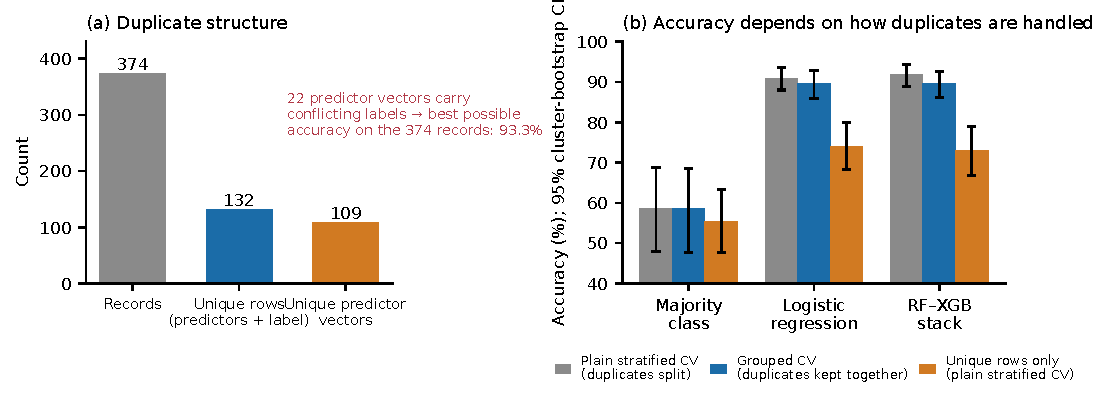
\includegraphics[width=\textwidth]{figs/fig2_audit.pdf}
\caption{(a) Record, unique-row and unique-predictor-vector counts. (b) Accuracy of the majority class, logistic regression and the RF--XGB stack under three protocols (10 repeated 5-fold CV; error bars are 95\% cluster-bootstrap CIs, see Section~\ref{sec:stats}).}\label{fig:audit}
\end{figure}

\subsection{Predictors}
Occupation was retained as a contextual predictor but may encode socioeconomic structure and transport poorly. The synonymous BMI labels ``Normal'' and ``Normal Weight'' were merged; blood pressure was split into systolic and diastolic values. Sleep duration and quality overlap conceptually with the definition of insomnia, so the predictor--outcome relation is partly circular; Section~\ref{sec:ablate} measures how much performance depends on them.

\section{Methods}\label{sec:methods}
\subsection{Models}
\textbf{Primary model (RF--XGB stack).} Algorithm~\ref{alg:stack} defines the primary two-learner stack. Preprocessing (standardisation of nine numeric predictors; one-hot encoding of gender, occupation and BMI category with the vocabulary taken from the training partition) is refitted inside every inner fold. The meta-learner is a multinomial logistic regression trained on $[\,x',\,p_{\mathrm{RF}},\,p_{\mathrm{XGB}}\,]$, where $x'$ is the encoded predictor vector passed through, and $p_{\mathrm{RF}},p_{\mathrm{XGB}}$ are out-of-fold class probabilities. Inner folds are stratified and \emph{group-aware}, so identical records never straddle an inner split. The base learners are refitted on the full training partition for inference. \textbf{Fixed configuration:} RF with 100 trees, depth 10, minimum split 5; XGBoost with 800 rounds, learning rate 0.02, depth 3, subsample/column sample 0.9, minimum child weight 3, $\gamma=0.15$, $\lambda=1.2$; meta-learner $C=2.0$. These values are taken from the earlier draft; their provenance cannot be verified, so Section~\ref{sec:nested} repeats the evaluation with all tuning inside the training partitions.

\begin{algorithm}[t]
\caption{Fold-isolated RF--XGB stacking (training partition $D_{tr}$, new record $x$)}\label{alg:stack}
\begin{algorithmic}[1]
\Require raw training data $(X_{tr},y_{tr})$; $K=5$ stratified, group-aware folds
\State Initialise out-of-fold matrices $P_{\mathrm{RF}},P_{\mathrm{XGB}}\in\mathbb{R}^{n_{tr}\times 3}$ and pass-through matrix $T$
\For{$k=1,\dots,K$}
  \State fit scaler and encoder $\tau_{-k}$ on the folds other than $k$ only
  \State fit RF and XGBoost on $\tau_{-k}(X_{-k})$; store their probabilities for fold $k$ in $P_{\mathrm{RF}},P_{\mathrm{XGB}}$
  \State store $\tau_{-k}(X_{k})$ in $T$ at the same row indices
\EndFor
\State fit multinomial logistic regression $g$ on $Z=[T,P_{\mathrm{RF}},P_{\mathrm{XGB}}]$ with labels $y_{tr}$
\State fit $\tau$, RF and XGBoost on all of $D_{tr}$
\State \Return $p(x)=g\big([\tau(x),\,f_{\mathrm{RF}}(\tau(x)),\,f_{\mathrm{XGB}}(\tau(x))]\big)$, $\ \hat y=\arg\max_c p_c(x)$
\end{algorithmic}
\end{algorithm}

\textbf{Comparators.} All comparators receive the same encoded training data: majority class; logistic regression ($C=1$); decision tree (depth 3); RF and XGBoost as configured above; soft voting, the unweighted mean of the \emph{same fitted} RF and XGBoost probabilities; and, as further competitive learners, extra trees, scikit-learn HistGradientBoosting, LightGBM \citep{ke2017}, CatBoost \citep{prokhorenkova2018}, an RBF SVM, and a two-layer MLP. The SVM appears only as an independent baseline; no analysis uses a three-learner stack. Hyper-parameters of these additional learners are modest fixed defaults (Appendix~A) and are not tuned, which disadvantages them on very small samples (Section~\ref{sec:cv}).

\subsection{Evaluation protocols}\label{sec:eval}
All protocols use 5-fold cross-validation repeated 10 times with different seeds, and every model is scored on identical outer splits (workflow in Appendix~B).
\begin{itemize}
\item \textbf{Grouped CV (primary).} Records with identical predictor vectors form a group; folds are stratified by class and grouped, so no predictor vector appears in both training and test folds (374 records).
\item \textbf{Plain stratified CV.} The same procedure without grouping, which lets duplicates fall on both sides of a split (the leakage-prone alternative).
\item \textbf{Unique rows.} The \NUnique{} unique rows only, with plain stratified splitting (a sensitivity analysis free of exact duplicates; \NConflictVec{} conflicting predictor vectors remain).
\item \textbf{Nested tuning.} For grouped CV and unique rows (5 repeats each), an inner 3-fold grouped CV on the outer-training partition selects the main hyper-parameter(s) of each model by log-loss (logistic $C\in\{0.1,1,10\}$; RF depth $\in\{3,6,10\}$; XGBoost rounds $\in\{200,800\}$; soft voting: RF depth and XGBoost rounds jointly; stack: XGBoost rounds and meta-learner $C\in\{0.1,1,10\}$, with RF depth fixed at 10 for cost). The outer test fold is never used for selection. For the unique-rows protocol the nested outer and inner splits are grouped by predictor vector, whereas the non-nested unique-rows analysis uses plain stratified splits, so Tables~\ref{tab:dedup} and~\ref{tab:nested} are not strictly like-for-like.
\item \textbf{Predictor ablation.} Grouped 10$\times$5-fold CV with the same fixed models after removing sleep duration and quality, and additionally stress level.
\item \textbf{Original split.} A re-implementation of the single stratified 80:20 split (seed 42; 299/75), including observation-level output.
\end{itemize}

\subsection{Metrics and statistical comparison}\label{sec:stats}
We report accuracy, macro-F1, macro one-vs-rest AUC \citep{fawcett2006}, multiclass Brier score \citep{brier1950}, log-loss and a five-bin equal-mass top-label expected calibration error (ECE$_5$; unstable at this sample size, so interpreted with caution) \citep{guo2017}. Repeat-level results are averaged over the 10 repeats. Confidence intervals for accuracy are \emph{cluster bootstrap} intervals (5{,}000 resamples of predictor-vector groups, applied to repeat-averaged correctness), which reflect sampling uncertainty of the data; the spread across repeats alone would understate it. For stack versus each comparator we report the mean accuracy difference with a 20{,}000-resample cluster-bootstrap interval, the Nadeau--Bengio corrected resampled $t$-test over the 50 fold-level differences \citep{nadeau2003}, and an exact McNemar test \citep{dietterich1998} in each repeat (median $p$ and the number of repeats with $p<0.05$). Single-split intervals are exact Clopper--Pearson intervals \citep{clopper1934}. We do not adjust for multiplicity; with 12 comparators, isolated nominal findings should be read as exploratory.

\subsection{Explanation analyses}
SHAP values were obtained with the permutation explainer \citep{lundberg2017}, using a 25-record background sampled from the training partition and 35 explanation records sampled from the test partition of the original split, with $2p+1$ evaluations ($p=25$ encoded features), on both the stack and the soft-voting model. The procedure was repeated 10 times with independent backgrounds and explanation samples; one-hot columns were summed per original predictor before taking absolute values, and importance is the mean of $|\phi|$ over records and classes. Stability is the mean pairwise Spearman correlation of the 12 importance values across runs and the Jaccard overlap of the top-3 sets. To examine collinearity we report Spearman correlations and variance-inflation factors on all 374 records, and a held-out permutation test (grouped 5-fold, 10 permutations) that shuffles a single predictor or a correlated block jointly and records the increase in log-loss. LIME \citep{ribeiro2016} was run in the encoded space (5{,}000 perturbations, 10 seeds) for four held-out records; for each we report the identifier, reference label, predicted probabilities, the weighted-surrogate $R^2$ (fidelity) and the rank agreement of weights across seeds.

\subsection{Software and reproducibility}
Python 3.13, scikit-learn 1.9.1 \citep{pedregosa2011}, XGBoost 3.4.1, LightGBM 4.7.0, CatBoost 1.2.10, SHAP 0.54.1, LIME 0.2.0.1, pandas 3.0.5, NumPy 2.5.3, SciPy 1.18.1. Seeds are fixed per repeat. The supplementary archive contains the complete code, a script that regenerates every table and in-text number from the stored results, the split identifiers (repeat, fold, row) for all protocols, and observation-level labels, predicted classes and class probabilities for every model, repeat and fold (Data and code availability).

\section{Results}
\subsection{Reproducing the original single hold-out}\label{sec:orig}
Re-running the documented specification on the original 80:20 split (seed 42) gave \OrigStackCorrect/75 correct for the stack (\OrigStackAcc\%, exact 95\% CI \OrigStackCPlo--\OrigStackCPhi\%; macro-F1 \OrigStackF) and \OrigVoteCorrect/75 for soft voting (Table~\ref{tab:orig}); using plain stratified rather than group-aware inner folds also gave 72/75. We were therefore \emph{unable to reproduce the 73/75 (97.33\%) reported in the earlier draft}, and we withdraw that figure; the original analysis code was not available for inspection. On this split the stack and soft voting differ on one record each way (McNemar $p=\OrigMcnemar$; paired bootstrap CI for the difference $\OrigBootLo$ to $+\OrigBootHi$ pp). Training accuracy is \OrigStackTrain\%, close to test accuracy, which is expected rather than reassuring: \OrigLeak{} of the 75 test records have a predictor vector that also occurs in the training set, so the test set largely re-asks questions the models have already seen. On the only \OrigNovel{} test records with unseen vectors the stack was correct on \OrigStackNovelCorrect, soft voting on \OrigVoteNovelCorrect, logistic regression on \OrigLRNovelCorrect{} (too few to compare). Fitted to all 374 records, RF and the stack reach \TrainAccRF\% and \TrainAccStack\% in-sample accuracy against the \Ceiling\% ceiling, which also explains the near-equal training and test accuracies (0.926 and 0.924) in the earlier repeated-split figure.

\begin{table}[t]\centering\small
\caption{Re-implementation of the single stratified 80:20 hold-out (seed 42). The last column counts test records whose predictor vector never occurs in the training set.}\label{tab:orig}
\resizebox{\textwidth}{!}{\begin{tabular}{@{}lcccccc@{}}
\toprule
Model & Correct/75 & Accuracy (\%) [exact 95\% CI] & Macro-F1 & Train acc.\ (\%) & Unseen-vector rows correct\\
\midrule
Logistic regression & 71 & 94.7 [86.9, 98.5] & 0.92 & 91.0 & 6/7\\
Random forest & 72 & 96.0 [88.8, 99.2] & 0.94 & 92.0 & 6/7\\
XGBoost & 70 & 93.3 [85.1, 97.8] & 0.89 & 91.6 & 4/7\\
Soft voting (RF+XGB) & 72 & 96.0 [88.8, 99.2] & 0.94 & 91.6 & 6/7\\
\textbf{Stacking (RF+XGB)} & 72 & 96.0 [88.8, 99.2] & 0.94 & 91.6 & 5/7\\
\bottomrule
\end{tabular}}
\end{table}

\subsection{Repeated duplicate-aware cross-validation}\label{sec:cv}
Table~\ref{tab:main} and Fig.~\ref{fig:models} give the primary results. The stack reached \AccStackG\% accuracy (95\% CI \CIloStackG--\CIhiStackG; fold-level SD \FoldSDStackG{} pp) and macro-F1 \FStackG. Every model with real capacity landed within about one point: soft voting \AccVoteG\%, random forest \AccRFG\%, XGBoost \AccXGBG\%, logistic regression \AccLRG\%, CatBoost \AccCatG\%, SVM \AccSVMG\%; a depth-3 tree reached \AccTreeG\% and the majority class \AccMajG\%. A shallow tree and a linear model recover almost everything because the table is dominated by a few templated patterns (occupation, BMI, blood pressure, age).

\begin{table}[t]\centering\small
\caption{Grouped repeated CV (10$\times$5-fold; 374 records; identical splits for all models; fixed hyper-parameters). Accuracy CIs are cluster-bootstrap; the other columns are means over 10 repeats.}\label{tab:main}
\resizebox{\textwidth}{!}{\begin{tabular}{@{}lcccccc@{}}
\toprule
Model & Accuracy (\%) [95\% CI] & Macro-F1 & Macro AUC & Brier & Log-loss & ECE$_5$\\
\midrule
Majority class & 58.6 [47.6, 68.6] & 0.25 & 0.50 & 0.571 & 0.966 & 0.006\\\midrule
Decision tree (depth 3) & 88.1 [84.1, 91.4] & 0.85 & 0.90 & 0.209 & 0.775 & 0.044\\
Logistic regression & 89.7 [86.0, 92.8] & 0.87 & 0.92 & 0.188 & 0.435 & 0.063\\
SVM (RBF) & 90.0 [86.7, 92.9] & 0.87 & 0.93 & 0.172 & 0.369 & 0.027\\\midrule
MLP (32,16) & 89.7 [86.5, 92.6] & 0.87 & 0.91 & 0.188 & 0.509 & 0.061\\
Random forest & 89.8 [86.4, 92.9] & 0.87 & 0.92 & 0.191 & 1.119 & 0.079\\
Extra trees & 88.7 [84.8, 92.0] & 0.86 & 0.92 & 0.207 & 1.337 & 0.075\\
HistGradientBoosting & 89.0 [85.6, 92.1] & 0.85 & 0.91 & 0.207 & 0.678 & 0.080\\
LightGBM & 89.5 [86.1, 92.5] & 0.86 & 0.91 & 0.204 & 0.648 & 0.088\\
CatBoost & 89.8 [86.3, 92.7] & 0.87 & 0.92 & 0.180 & 0.397 & 0.045\\\midrule
XGBoost & 89.8 [86.3, 92.9] & 0.87 & 0.92 & 0.185 & 0.431 & 0.055\\
Soft voting (RF+XGB) & 89.8 [86.3, 92.9] & 0.87 & 0.92 & 0.184 & 0.447 & 0.060\\
\textbf{Stacking (RF+XGB)} & 89.6 [86.1, 92.7] & 0.87 & 0.91 & 0.186 & 0.446 & 0.062\\
\bottomrule
\end{tabular}}
\end{table}

\begin{figure}[t]
\centering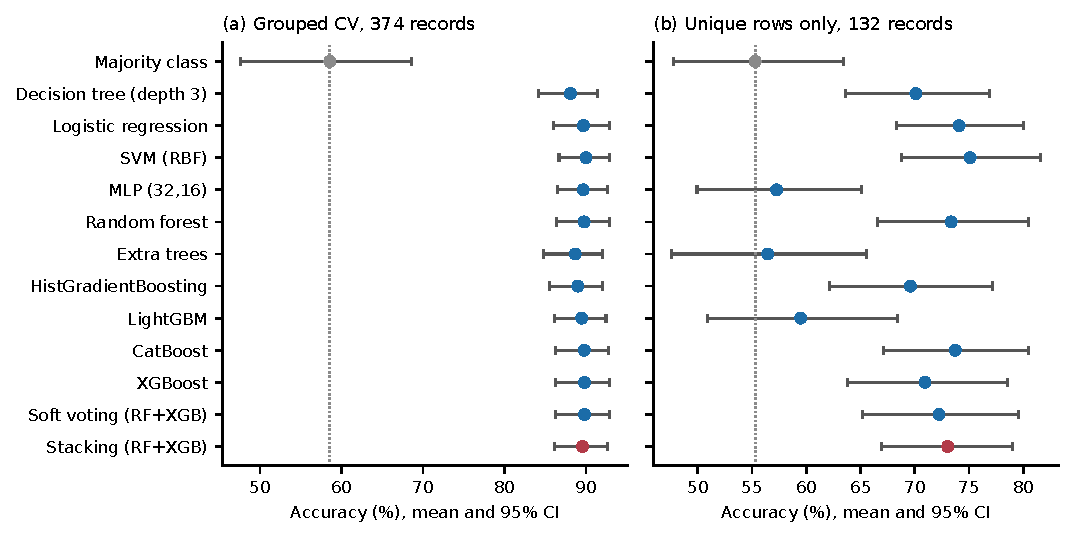
\includegraphics[width=\textwidth]{figs/fig3_models.pdf}
\caption{Accuracy of all models under grouped CV (a) and on the unique rows (b). Points are 10-repeat means; bars are 95\% cluster-bootstrap CIs; the dotted line is the majority-class accuracy. The stack is shown in red.}\label{fig:models}
\end{figure}

\textbf{Protocol effects.} Plain stratified CV, which lets duplicates straddle splits, raised the stack's accuracy to \AccStackN\% (\InflationNaiveGrouped{} points above grouped CV). On the \NUnique{} unique rows the stack reached \AccStackD\% (CI in Table~\ref{tab:dedup}), \DropGroupedDedup{} points below grouped CV, against \AccMajD\% for the majority class; logistic regression reached \AccLRD\%. Several untuned learners (extra trees, LightGBM, the MLP) fell to near majority-class accuracy on 132 rows, a reminder that default settings do not transfer to very small samples. Performance on this table is thus largely a function of how duplicates are treated.

\begin{table}[t]\centering\small
\caption{Repeated CV on the \NUnique{} unique rows only (plain stratified 5-fold, 10 repeats). Same format as Table~\ref{tab:main}.}\label{tab:dedup}
\begin{tabular}{@{}lcccc@{}}
\toprule
Model & Accuracy (\%) [95\% CI] & Macro-F1 & Brier & Log-loss\\
\midrule
Majority class & 55.3 [47.7, 63.4] & 0.24 & 0.594 & 0.998\\\midrule
Decision tree (depth 3) & 70.1 [63.6, 76.9] & 0.64 & 0.488 & 2.904\\
Logistic regression & 74.1 [68.3, 80.0] & 0.68 & 0.435 & 0.838\\
SVM (RBF) & 75.1 [68.7, 81.6] & 0.68 & 0.405 & 0.740\\\midrule
MLP (32,16) & 57.3 [49.9, 65.1] & 0.52 & 0.723 & 3.316\\
Random forest & 73.4 [66.6, 80.5] & 0.66 & 0.482 & 1.885\\
Extra trees & 56.4 [47.6, 65.5] & 0.48 & 0.808 & 9.056\\
HistGradientBoosting & 69.6 [62.2, 77.2] & 0.63 & 0.515 & 1.126\\
LightGBM & 59.5 [50.9, 68.4] & 0.52 & 0.726 & 1.837\\
CatBoost & 73.7 [67.1, 80.5] & 0.67 & 0.460 & 0.862\\\midrule
XGBoost & 70.9 [63.8, 78.5] & 0.64 & 0.486 & 0.941\\
Soft voting (RF+XGB) & 72.2 [65.2, 79.6] & 0.65 & 0.478 & 0.977\\
\textbf{Stacking (RF+XGB)} & 73.0 [66.9, 79.0] & 0.67 & 0.452 & 0.900\\
\bottomrule
\end{tabular}
\end{table}

\subsection{Paired comparisons}\label{sec:paired}
Table~\ref{tab:paired} and Fig.~\ref{fig:paired} test the stack against every comparator. Against soft voting under grouped CV the mean difference is \DiffVoteG{} pp (95\% CI \DiffLoVoteG{} to \DiffHiVoteG; median McNemar $p=\McnPVoteG$; stack better, tied and worse in \FoldsBetterVote/\FoldsTieVote/\FoldsWorseVote{} of 50 folds; on average \VoteDiscStack{} records were correct only under the stack and \VoteDiscVote{} only under soft voting). Differences against logistic regression (\DiffLRG{} pp, CI \DiffLoLRG{} to \DiffHiLRG), RF (\DiffRFG{}) and XGBoost (\DiffXGBG{}) are likewise indistinguishable from zero; apart from the majority-class baseline, the only interval that excludes zero is that against the \SigGrouped{}, a deliberately weak baseline. On unique rows the intervals are wider and include zero for all competitive learners (extra trees, LightGBM and the MLP are worse than the stack, but they are untuned and fall to near majority-class accuracy; against soft voting: \DiffVoteD{} pp, CI \DiffLoVoteD{} to \DiffHiVoteD). \emph{The stack is not superior to soft voting, to its own base learners, or to logistic regression on this dataset.}

\begin{table}[t]\centering\small
\caption{Stack minus comparator, accuracy difference in percentage points with cluster-bootstrap 95\% CI; fold-level wins/ties/losses out of 50; per-repeat exact McNemar tests; Nadeau--Bengio corrected $t$-test. No multiplicity correction.}\label{tab:paired}
\resizebox{\textwidth}{!}{\begin{tabular}{@{}lccccc@{}}
\toprule
Comparator & $\Delta$ accuracy (pp) [95\% CI] & Folds: stack $>$/=/$<$ & Median McNemar $p$ & Repeats $p<0.05$ & Corrected $t$-test $p$\\
\midrule
\multicolumn{6}{@{}l}{\textit{Grouped CV (374 records)}}\\
Majority class & +31.0 [+20.7, +41.8] & 50/0/0 & $<$0.001 & 10/10 & $<$0.001\\
Decision tree (depth 3) & +1.5 [+0.4, +3.0] & 29/14/7 & 0.18 & 1/10 & 0.73\\
Logistic regression & -0.1 [-1.2, +0.9] & 12/24/14 & 1.00 & 0/10 & 0.98\\
SVM (RBF) & -0.4 [-2.0, +0.8] & 12/16/22 & 0.59 & 1/10 & 0.93\\
MLP (32,16) & -0.1 [-0.9, +0.7] & 13/16/21 & 0.48 & 0/10 & 0.98\\
Random forest & -0.2 [-1.6, +1.2] & 16/16/18 & 0.90 & 0/10 & 0.97\\
Extra trees & +0.9 [-0.2, +2.2] & 23/14/13 & 0.53 & 2/10 & 0.85\\
HistGradientBoosting & +0.6 [-1.2, +2.3] & 21/12/17 & 0.24 & 1/10 & 0.93\\
LightGBM & +0.1 [-1.4, +1.4] & 11/24/15 & 0.32 & 0/10 & 0.99\\
CatBoost & -0.2 [-1.6, +1.1] & 14/19/17 & 0.68 & 0/10 & 0.96\\
XGBoost & -0.2 [-1.8, +1.2] & 14/19/17 & 0.77 & 1/10 & 0.95\\
Soft voting (RF+XGB) & -0.2 [-1.8, +1.1] & 15/17/18 & 0.68 & 0/10 & 0.95\\
\midrule
\multicolumn{6}{@{}l}{\textit{Unique rows only (132 records)}}\\
Majority class & +17.7 [+10.7, +25.2] & 48/1/1 & $<$0.001 & 10/10 & 0.31\\
Decision tree (depth 3) & +3.0 [-0.2, +6.3] & 30/6/14 & 0.40 & 2/10 & 0.88\\
Logistic regression & -1.1 [-2.3, +0.1] & 9/23/18 & 1.00 & 1/10 & 0.92\\
SVM (RBF) & -2.0 [-4.8, +0.7] & 11/18/21 & 0.75 & 2/10 & 0.85\\
MLP (32,16) & +15.8 [+12.0, +19.5] & 45/4/1 & $<$0.001 & 10/10 & 0.51\\
Random forest & -0.3 [-3.3, +2.6] & 17/15/18 & 0.54 & 0/10 & 0.98\\
Extra trees & +16.7 [+11.8, +21.2] & 48/0/2 & $<$0.001 & 10/10 & 0.45\\
HistGradientBoosting & +3.5 [-0.3, +7.4] & 30/9/11 & 0.47 & 1/10 & 0.83\\
LightGBM & +13.6 [+8.5, +18.6] & 45/1/4 & 0.001 & 9/10 & 0.53\\
CatBoost & -0.7 [-3.6, +2.2] & 18/10/22 & 1.00 & 0/10 & 0.96\\
XGBoost & +2.1 [-1.8, +6.1] & 28/6/16 & 0.33 & 0/10 & 0.90\\
Soft voting (RF+XGB) & +0.8 [-2.8, +4.5] & 21/13/16 & 0.42 & 0/10 & 0.96\\
\bottomrule
\end{tabular}}
\end{table}

\begin{figure}[t]
\centering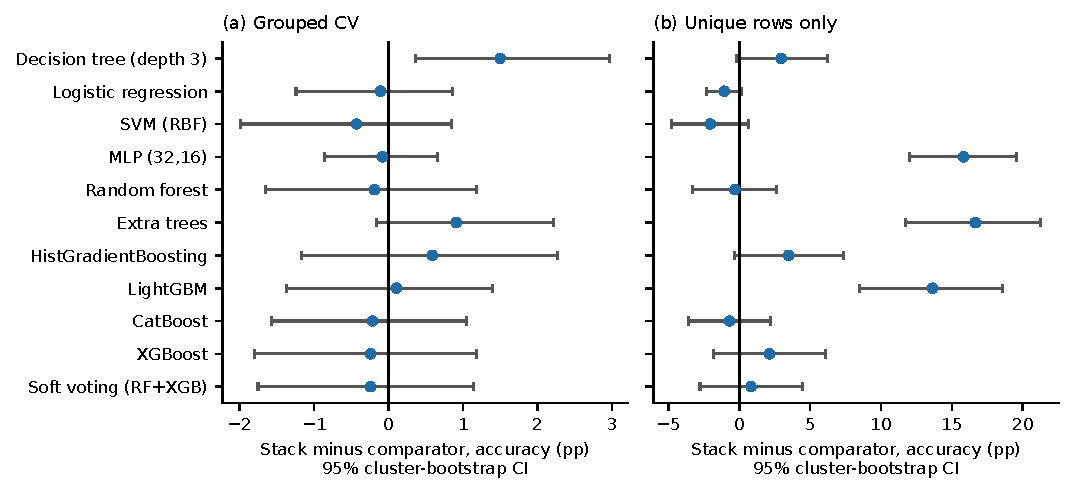
\includegraphics[width=\textwidth]{figs/fig4_paired.pdf}
\caption{Accuracy difference (stack minus comparator) with 95\% cluster-bootstrap CI under grouped CV (a) and on unique rows (b). Positive values favour the stack.}\label{fig:paired}
\end{figure}

\subsection{Nested tuning}\label{sec:nested}
When all hyper-parameter selection is confined to inner folds of the training partition, the picture is unchanged (Table~\ref{tab:nested}). Under grouped CV the stack reaches \NAccStackG\% (CI \NCIloStackG--\NCIhiStackG), soft voting \NAccVoteG\%, XGBoost \NAccXGBG\%, RF \NAccRFG\% and logistic regression \NAccLRG\%. The stack minus soft voting difference is \NDiffVoteG{} pp (CI \NDiffLoVoteG{} to \NDiffHiVoteG); minus XGBoost \NDiffXGBG{} (\NDiffLoXGBG{} to \NDiffHiXGBG); minus logistic regression \NDiffLRG{} (\NDiffLoLRG{} to \NDiffHiLRG); minus RF \NDiffRFG{} (\NDiffLoRFG{} to \NDiffHiRFG). The RF interval narrowly excludes zero, an isolated nominal result among eight comparisons that we do not interpret as evidence of an advantage. On unique rows the stack reaches \NAccStackD\% (\NCIloStackD--\NCIhiStackD) with every paired interval including zero except logistic regression (\NDiffLRD{} pp; \NDiffLoLRD{} to \NDiffHiLRD), and no repeat-level McNemar test was significant in any comparison. Selection sat at the lower edge of the grid in nearly every fold (RF depth 3 and XGBoost with 200 rounds in all 25 outer folds in both protocols; logistic $C=0.1$ in most), so tuning acted mainly as extra regularisation, and a wider grid might select differently.

\begin{table}[t]\centering\small
\caption{Repeated nested CV (5 repeats $\times$ 5 outer folds; inner 3-fold grouped selection on training partitions only).}\label{tab:nested}
\begin{tabular}{@{}lcccc@{}}
\toprule
Model & Accuracy (\%) [95\% CI] & Macro-F1 & Brier & Log-loss\\
\midrule
\multicolumn{5}{@{}l}{\textit{Grouped CV (374 records)}}\\
Logistic regression & 89.0 [85.3, 92.4] & 0.86 & 0.198 & 0.428\\
Random forest & 89.2 [85.5, 92.5] & 0.86 & 0.181 & 0.385\\
XGBoost & 90.1 [86.7, 93.2] & 0.87 & 0.175 & 0.378\\
Soft voting (RF+XGB) & 89.9 [86.5, 93.0] & 0.87 & 0.175 & 0.374\\
\textbf{Stacking (RF+XGB)} & 90.0 [86.6, 93.1] & 0.87 & 0.184 & 0.399\\
\midrule
\multicolumn{5}{@{}l}{\textit{Unique rows only (132 records)}}\\
Logistic regression & 75.0 [69.0, 81.0] & 0.70 & 0.415 & 0.755\\
Random forest & 76.7 [70.6, 82.9] & 0.71 & 0.394 & 0.730\\
XGBoost & 76.9 [70.7, 83.2] & 0.71 & 0.394 & 0.737\\
Soft voting (RF+XGB) & 76.5 [70.4, 82.5] & 0.71 & 0.390 & 0.725\\
\textbf{Stacking (RF+XGB)} & 77.2 [71.5, 83.2] & 0.72 & 0.406 & 0.741\\
\bottomrule
\end{tabular}
\end{table}

\subsection{Probability calibration}\label{sec:calib}
Fig.~\ref{fig:calib} shows reliability and Brier scores for grouped CV. Brier scores (lower is better) are similar for the stack (\BrierStackG), soft voting (\BrierVoteG), XGBoost (\BrierXGBG) and logistic regression (\BrierLRG); the SVM and CatBoost were best (\BrierSVMG, \BrierCatG). Log-loss is similar for XGBoost (\LlXGBG), logistic regression (\LlLRG), the stack (\LlStackG) and soft voting (\LlVoteG), and best for the SVM (\LlSVMG) and CatBoost (\LlCatG). Random forest stands out (\LlRFG) because it assigns exactly zero probability to the true class for about 3\% of held-out predictions, which log-loss penalises heavily; averaging with XGBoost removes this in soft voting and stacking. ECE$_5$ was \EceStackG{} for the stack and \EceVoteG{} for soft voting. No post-hoc recalibration was applied, and the five-bin estimate is noisy.

\begin{figure}[t]
\centering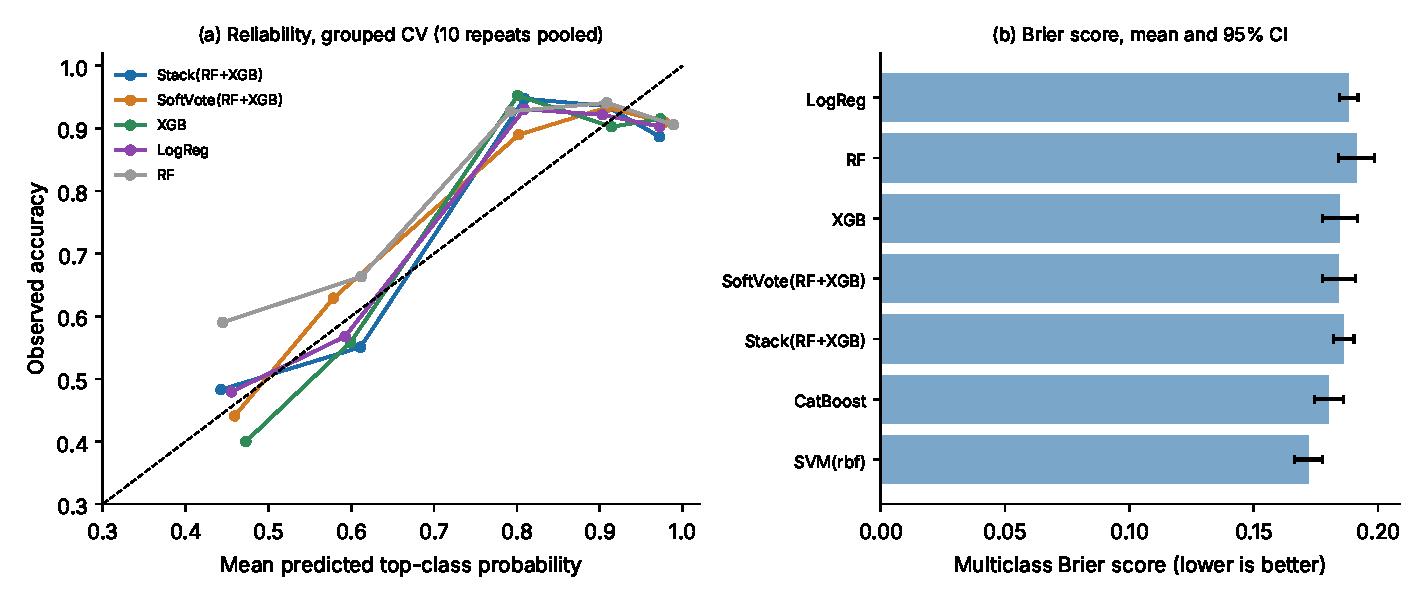
\includegraphics[width=\textwidth]{figs/fig5_calibration.pdf}
\caption{(a) Reliability of top-class probabilities (bins with at least 20 predictions; 10 grouped-CV repeats pooled). (b) Multiclass Brier score, mean and 95\% $t$-interval across repeats.}\label{fig:calib}
\end{figure}

\subsection{Dependence on sleep-behaviour predictors}\label{sec:ablate}
Removing sleep duration and quality, or additionally stress, barely changes accuracy (Table~\ref{tab:ablate}). The signal is carried by other predictors (occupation, BMI, blood pressure, age), which is consistent with templated generation. The conceptual overlap between sleep duration/quality and insomnia is therefore not what drives the benchmark accuracy, although it would matter for any genuine deployment.

\begin{table}[t]\centering\small
\caption{Grouped repeated CV accuracy (\%, 10 repeats) after removing sleep-behaviour predictors.}\label{tab:ablate}
\begin{tabular}{@{}lccc@{}}
\toprule
Predictor set & Stacking & Soft voting & Logistic regression\\
\midrule
All predictors & 89.6 & 89.8 & 89.7\\
Without sleep duration \& quality & 89.9 & 89.9 & 89.1\\
Without sleep duration, quality \& stress & 89.2 & 89.9 & 88.9\\
\bottomrule
\end{tabular}
\end{table}

\subsection{Explanation stability, collinearity and local audit}\label{sec:xai}
\textbf{Stability.} Across 10 independent backgrounds and explanation samples, SHAP importance rankings were highly reproducible within an architecture (mean pairwise rank correlation \ShapRhoStack{} for stacking, \ShapRhoVote{} for soft voting; minimum \ShapMinRhoStack{} and \ShapMinRhoVote), although top-3 sets were less stable (Jaccard \ShapJacStack{} and \ShapJacVote; Table~\ref{tab:shap}, Fig.~\ref{fig:shap}). Reproducible within a model does not mean the same across models: the mean importance profiles of stacking and soft voting correlate only weakly ($\rho=\ShapStackVote$).

\begin{table}[t]\centering\small
\caption{SHAP stability and collinearity diagnostics for the stack and the soft-voting model (original-split training partition; explanation sample 35 test records; 10 runs).}\label{tab:shap}
\resizebox{\textwidth}{!}{\begin{tabular}{@{}lcc@{}}
\toprule
Quantity & Stacking & Soft voting\\
\midrule
Mean pairwise rank correlation across 10 runs (min) & 0.98 (0.94) & 0.97 (0.94)\\
Mean pairwise Jaccard overlap of top-3 sets & 0.73 & 0.72\\
Top-3 predictors (mean $|\phi|$) & Diastolic BP, Occupation, Sleep Duration & Systolic BP, BMI Category, Physical Activity Level\\
Blood-pressure block, mean $|\phi|$ (SBP+DBP) & 0.148 & 0.156\\
Sleep/stress block (duration+quality+stress) & 0.148 & 0.054\\
Activity block (activity+steps) & 0.080 & 0.058\\
Held-out $\Delta$log-loss, SBP / DBP alone & 0.125 / 0.298 & 0.136 / 0.015\\
Held-out $\Delta$log-loss, BP block permuted jointly & 0.647 & 0.318\\
\bottomrule
\end{tabular}}
\end{table}

\begin{figure}[t]
\centering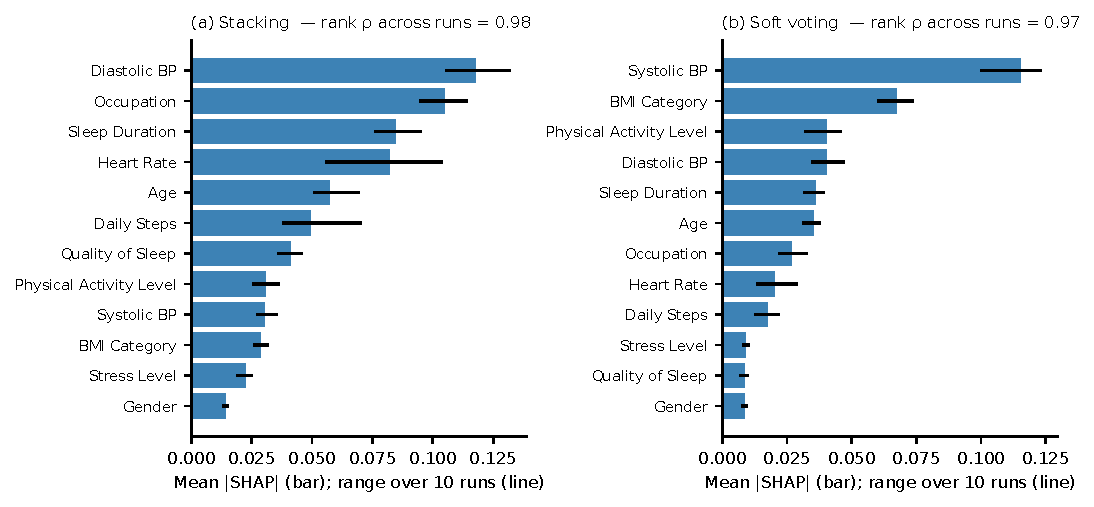
\includegraphics[width=\textwidth]{figs/fig6_shap.pdf}
\caption{Global SHAP importance (mean $|\phi|$ summed over one-hot columns) for the stack (a) and soft voting (b). Bars: mean over 10 runs; lines: range over runs. Orderings differ between panels.}\label{fig:shap}
\end{figure}

\textbf{Collinearity.} The predictors are strongly dependent (Spearman: systolic--diastolic \RhoBP; sleep duration--quality \RhoSleepQual; quality--stress \RhoQualStress; activity--steps \RhoActSteps; variance-inflation factors \VIFSystolicBP{} and \VIFDiastolicBP{} for systolic and diastolic pressure, \VIFQualityofSleep{} for quality of sleep). The stack passes encoded predictors to a linear meta-learner, whereas soft voting uses trees only, and the two attribute importance differently: soft voting concentrates it on systolic pressure, whereas the stack spreads it across diastolic pressure, occupation, sleep duration and heart rate. The blood-pressure \emph{pair}, however, receives almost the same total attribution under both architectures (\BlockBPStack{} versus \BlockBPVote), and permuting the pair jointly on held-out data increases log-loss far more than permuting either member alone (stack: \PermBPblockStack{} versus \PermSBPStack{} and \PermDBPStack; soft voting: \PermBPblockVote{} versus \PermSBPVote{} and \PermDBPVote). In other words, the architectures disagree about \emph{which} of two near-duplicate variables to credit, not about whether blood pressure matters; single-variable rankings of correlated predictors should not be interpreted individually. The sleep/stress block, in contrast, differs between architectures (\BlockSleepStack{} versus \BlockSleepVote), because the linear meta-learner uses these predictors directly whereas the trees barely do.

\textbf{Local audit.} Table~\ref{tab:lime} identifies each explained record by Person ID, with its reference label, predicted probabilities and surrogate fidelity. LIME $R^2$ was \LimeRsqStackMin--\LimeRsqStackMax{} for the stack and \LimeRsqVoteMin--\LimeRsqVoteMax{} for soft voting: good for the stack and clearly weaker for soft voting, whose local surrogate should therefore be read more cautiously. Rank agreement of weights across seeds was at least \LimeRhoStackMin{} for the stack. The record with Person ID 84 is a ``None'' record predicted with probability only 0.38 by the stack, and Person ID 19 is a misclassified insomnia record (predicted apnea with probability 0.67 by both models). Local explanations differ between architectures for the same record, as the global ones do.

\begin{table}[t]\centering\small
\caption{Audited local explanations (original-split test records). Person ID is the dataset identifier; $R^2$ is LIME's weighted-surrogate fidelity (mean of 10 seeds); rank $\rho$ is the mean pairwise Spearman correlation of absolute weights across seeds; top-3 features by mean weight in the encoded space.}\label{tab:lime}
\resizebox{\textwidth}{!}{\begin{tabular}{@{}llllcccl@{}}
\toprule
Model & Person ID & Reference & Predicted & $P$(Ins./None/Apnea) & LIME $R^2$ & Rank $\rho$ & Top-3 local features\\
\midrule
Stacking & 244 & Insomnia & Insomnia & 0.90/0.08/0.02 & 0.77 & 0.98 & Sleep Duration, Age, Diastolic BP\\
Soft voting & 244 & Insomnia & Insomnia & 0.97/0.03/0.00 & 0.51 & 0.82 & Systolic BP, Physical Activity Level, Sleep Duration\\\midrule
Stacking & 84 & None & None & 0.32/0.38/0.30 & 0.79 & 0.98 & Diastolic BP, Heart Rate, Age\\
Soft voting & 84 & None & None & 0.07/0.84/0.08 & 0.64 & 0.84 & Systolic BP, Diastolic BP, BMI Category Normal\\\midrule
Stacking & 291 & Sleep Apnea & Sleep Apnea & 0.06/0.05/0.89 & 0.76 & 0.97 & Heart Rate, Sleep Duration, Diastolic BP\\
Soft voting & 291 & Sleep Apnea & Sleep Apnea & 0.02/0.08/0.91 & 0.60 & 0.85 & Systolic BP, Age, Diastolic BP\\\midrule
Stacking & 19 & Insomnia & Sleep Apnea & 0.08/0.25/0.67 & 0.76 & 0.97 & Heart Rate, Sleep Duration, Diastolic BP\\
Soft voting & 19 & Insomnia & Sleep Apnea & 0.28/0.05/0.67 & 0.60 & 0.81 & Systolic BP, Age, Diastolic BP\\
\bottomrule
\end{tabular}}
\end{table}

\section{Discussion}
\textbf{Principal findings.} On this benchmark, a leakage-controlled RF--XGB stack achieves roughly 90\% accuracy under duplicate-aware validation, but so do a logistic regression, a shallow tree (within about 1.5 points) and every competitive tree or kernel learner. Stacking brings no measurable gain over soft voting, its own base learners or the linear baseline, neither in accuracy nor in calibration. The one-observation difference in the earlier draft was not evidence of an advantage and, as we now show, the headline figure itself was not reproducible.

\textbf{Why the earlier estimate was optimistic.} Three mechanisms compound: duplicated rows allow memorisation across a random split (\OrigLeak{} of 75 test records here); a single 75-record split has an exact 95\% interval of roughly \OrigStackCPlo--\OrigStackCPhi\%; and fixed hyper-parameters of unverifiable origin were used. Accuracy on unique rows (\AccStackD\% for the stack) is a fairer indication of how the models behave on records they have not effectively seen, and even that remains conditional on a dataset with conflicting labels. Because the file caps attainable accuracy at \Ceiling\%, near-ceiling accuracy on it indicates memorisation of its generating patterns, not clinical signal.

\textbf{Statistical power.} With 75 test records, the single-split comparison between stack and soft voting rests on two discordant records; an exact McNemar test cannot reject with so few discordant pairs, and at the observed discordance rate the smallest difference detectable with 80\% power is about \OrigMDE{} points, four times the one-record (1.33-point) difference reported in the earlier draft. Detecting a true 1.33-point difference at that discordance rate would require roughly \NReq{} test records, more than three times the entire dataset. Even the repeated, paired analysis here uses 374 correlated records and \NVec{} distinct predictor vectors, so its intervals (about $\pm1.5$ pp for most comparisons) cannot exclude advantages or disadvantages of that size. The correct reading is ``no evidence of a difference'', not ``evidence of no difference''.

\textbf{Collinearity and explanations.} Section~\ref{sec:xai} shows that attribution rankings of correlated predictors are architecture-specific while block-level attribution is stable. Single-variable SHAP or LIME rankings should therefore be reported together with the correlation structure and, where possible, block-level or grouped permutation importance. Neither technique establishes biological or clinical mechanism: SHAP, LIME and permutation importance describe the behaviour of a fitted function on this data distribution \citep{kumar2020,jung2023}.

\textbf{Benchmark outcomes versus clinical screening.} A reader should not treat any figure in this paper as diagnostic evidence. The labels come from an undocumented source without clinical adjudication; the task is reproducing a recorded category from lifestyle and cardiometabolic variables, which is not screening. Real-world screening would require prospectively collected participants with polysomnography or clinician-confirmed outcomes, pre-specified intended use and thresholds, evaluation of sensitivity and specificity at clinically meaningful operating points, calibration in the target population, subgroup performance, and external validation \citep{collins2024tripod,riley2024,lekadir2025}. A model that reproduces a benchmark's labels, even perfectly, may carry no clinical information if those labels were generated by simple rules.

\textbf{Contribution and novelty.} Stacking RF and XGBoost with a logistic meta-learner is standard practice, as are SHAP and LIME; we claim no new algorithm. What this work offers is a verified, leakage-controlled implementation, a quantified account of how duplicate structure and single splits inflate estimates on a widely used benchmark, a like-for-like comparison against simple and recent learners with paired statistics and calibration, and an explanation audit including collinearity and stability. Its practical message is that simple baselines and duplicate checks should precede any claim of ensemble benefit on small tabular health datasets \citep{rudin2019}.

\section{Limitations}
(i) The data have no documented provenance and appear templated; results do not generalise to patient populations. (ii) The meaning of the ``None'' label is undocumented. If ``None'' means ``no disorder recorded'' rather than ``clinically excluded'', the 219 records may contain undiagnosed cases; any classifier then learns to predict the \emph{recording} of a disorder, and class-conditional errors (especially false ``None'' predictions) are biased towards under-detection in ways this dataset cannot quantify. Treating these records as missing instead would discard 59\% of the sample and change the task. (iii) Duplicates and label conflicts impose a ceiling and make group-aware evaluation necessary; the unique-rows analysis retains conflicting vectors. (iv) The sample is small, so even the repeated analyses have wide intervals and repeated splits are not independent; the Nadeau--Bengio correction is approximate and no multiplicity adjustment is applied. (v) The additional learners use fixed, untuned settings. Pretrained tabular foundation models and attention-based tabular networks \citep{hollmann2025} were not evaluated because pretrained weights were unavailable in our environment, and they would be unlikely to be informative on \NVec{} distinct vectors. (vi) Explanations describe fitted models only. (vii) ECE is unstable at this sample size. (viii) No external cohort was available.

\section{Future work}
We recommend (a) external validation on a clinically characterised cohort with adjudicated outcomes and polysomnography-based reference standards, with calibration assessed in that population; (b) repeated nested cross-validation, calibration assessment and paired testing as the default for small tabular studies (applied here); (c) pre-registered sample-size justification for comparisons between ensembles; and (d) a minimum reporting standard for local explanations: the observation identifier, reference label, predicted class probabilities, explainer settings (background size, number of perturbations, kernel width, seeds), surrogate fidelity and stability across seeds, as in Table~\ref{tab:lime}. Evaluating tabular foundation models and tuned neural networks once pretrained weights are available is a natural extension.

\section{Conclusion}
After verifying outcome coding, removing duplicate leakage from the evaluation and comparing models under identical repeated splits, RF--XGB stacking performs at about the same level as soft voting, its base learners and logistic regression on the Sleep Health and Lifestyle Dataset (\AccStackG\% accuracy under grouped CV; \AccStackD\% on unique rows). The earlier single-split result (97.33\%) was not reproducible and overstated performance. SHAP rankings are reproducible within a model but architecture-dependent for correlated predictors. These findings concern a computational benchmark; they say nothing about diagnostic validity.

\section*{Declarations}
\small
\textbf{Data and code availability.} The dataset is publicly available on Kaggle \citep{kaggle}; reuse is subject to the platform's licence and terms, so the file itself is not redistributed (its SHA-256 and row count are checked by the code). The supplementary archive contains the code, software versions, seeds, split identifiers for all protocols, observation-level reference labels, predicted classes and class probabilities for every model, repeat and fold, the SHAP and LIME run outputs, and the scripts that regenerate every table and in-text number.\\
\textbf{Ethics.} Secondary computational analysis of a public dataset; no participants were recruited or contacted and no new human or animal data were collected. Person ID is used only to cite audited records.\\
\textbf{Funding.} This research received no specific grant from funding agencies in the public, commercial or not-for-profit sectors.\\
\textbf{Declaration of competing interest.} The authors declare no known competing financial interests or personal relationships that could have influenced the work reported here.\\
\textbf{Declaration of generative AI and AI-assisted technologies in the manuscript preparation process.} During the preparation of this work the authors used AI assistants (Claude, Anthropic) to assist with code development for the revision analyses, manuscript editing and LaTeX formatting. The authors reviewed and edited the output and take full responsibility for the content of the publication.\\
\textbf{Author contributions.} [To be completed by the authors.]
\normalsize

\appendix
\section{Hyper-parameters of all models}
\begin{table}[h]\centering\small
\caption{Fixed configurations (all other settings are library defaults). Seeds: $1000+$repeat index for repeated CV and the predictor ablation, $2000+$repeat index for nested CV, the repeat index for outer splits, 42 for the original split, 7 (with per-run seeds) for SHAP and 0--9 for LIME; see code.}
\begin{tabular}{@{}lp{11.8cm}@{}}
\toprule Model & Configuration\\\midrule
Logistic regression & multinomial, L2, $C=1$, lbfgs, max 5000 iterations\\
Decision tree & depth 3\\
Random forest & 100 trees, depth 10, min.\ split 5, min.\ leaf 1\\
XGBoost & 800 rounds, learning rate 0.02, depth 3, subsample 0.9, colsample 0.9, min.\ child weight 3, $\gamma=0.15$, $\lambda=1.2$, hist\\
Soft voting & mean of the fitted RF and XGBoost probabilities\\
Stack & RF and XGBoost as above; 5 stratified group-aware inner folds; meta-learner multinomial logistic, $C=2.0$, inputs $[$encoded $x$, $p_{\mathrm{RF}}$, $p_{\mathrm{XGB}}]$\\
Extra trees & 300 trees\\
HistGradientBoosting & 200 iterations, learning rate 0.05\\
LightGBM & 300 rounds, learning rate 0.05, 8 leaves, min.\ child samples 5\\
CatBoost & 300 iterations, depth 4, learning rate 0.05\\
MLP & hidden layers (32, 16), $\alpha=10^{-3}$, max 3000 iterations\\
SVM & RBF, $C=2$, Platt probabilities\\\bottomrule
\end{tabular}
\end{table}

\section{Workflow}
\begin{figure}[h]
\centering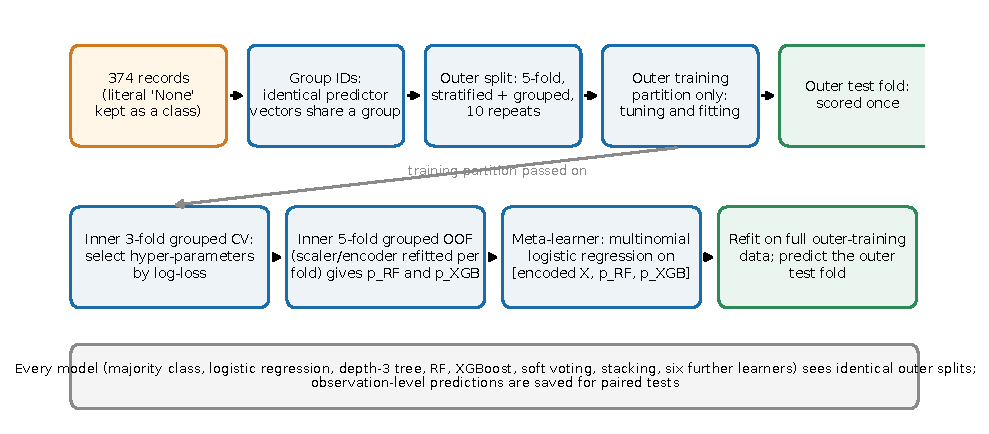
\includegraphics[width=\textwidth]{figs/fig1_protocol.pdf}
\caption{Evaluation workflow for the repeated nested protocol. Grouping, outer splitting, inner tuning, fold-isolated preprocessing and outer-fold scoring are applied identically to every model.}\label{fig:protocol}
\end{figure}

\small
\begin{thebibliography}{99}
\bibitem[Abd-alrazaq et al.(2024)]{abdalrazaq2024} Abd-alrazaq A, Aslam H, AlSaad R, Alsahli M, Ahmed A et al. Detection of sleep apnea using wearable AI: systematic review and meta-analysis. J Med Internet Res 2024; 26: e58187. doi: 10.2196/58187.
\bibitem[Alom et al.(2024)]{alom2024} Alom MS, Jeba SM, Debnath A, Aurpa TT, Siddiqua R. Enhancing sleep disorder diagnosis with a machine learning approach using ensemble neural networks. In: Proc.\ 11th Int.\ Conf.\ Networking, Systems, and Security; 2024. pp.\ 48--55. doi: 10.1145/3704522.3704533.
\bibitem[Bazoukis et al.(2023)]{bazoukis2023} Bazoukis G, Bollepalli SC, Chung CT, Li X, Tse G et al. Application of artificial intelligence in the diagnosis of sleep apnea. J Clin Sleep Med 2023; 19(7): 1337--1363. doi: 10.5664/jcsm.10532.
\bibitem[Borisov et al.(2024)]{borisov2024} Borisov V, Leemann T, Se{\ss}ler K, Haug J, Pawelczyk M et al. Deep neural networks and tabular data: a survey. IEEE Trans Neural Netw Learn Syst 2024; 35(6): 7499--7519. doi: 10.1109/TNNLS.2022.3229161.
\bibitem[Brier(1950)]{brier1950} Brier GW. Verification of forecasts expressed in terms of probability. Mon Weather Rev 1950; 78(1): 1--3.
\bibitem[Clopper and Pearson(1934)]{clopper1934} Clopper CJ, Pearson ES. The use of confidence or fiducial limits illustrated in the case of the binomial. Biometrika 1934; 26(4): 404--413.
\bibitem[Collins et al.(2024a)]{collins2024tripod} Collins GS, Moons KGM, Dhiman P, Riley RD, Beam AL et al. TRIPOD+AI statement: updated guidance for reporting clinical prediction models that use regression or machine learning methods. BMJ 2024; 385: e078378. doi: 10.1136/bmj-2023-078378.
\bibitem[Collins et al.(2024b)]{collins2024eval} Collins GS, Dhiman P, Ma J, Schlussel MM, Archer L et al. Evaluation of clinical prediction models (part 1): from development to external validation. BMJ 2024; 384: e074819. doi: 10.1136/bmj-2023-074819.
\bibitem[Dietterich(1998)]{dietterich1998} Dietterich TG. Approximate statistical tests for comparing supervised classification learning algorithms. Neural Comput 1998; 10(7): 1895--1923.
\bibitem[Efthimiou et al.(2024)]{efthimiou2024} Efthimiou O, Seo M, Chalkou K, Debray T, Egger M et al. Developing clinical prediction models: a step-by-step guide. BMJ 2024; 386: e078276. doi: 10.1136/bmj-2023-078276.
\bibitem[Fawcett(2006)]{fawcett2006} Fawcett T. An introduction to ROC analysis. Pattern Recognit Lett 2006; 27(8): 861--874. doi: 10.1016/j.patrec.2005.10.010.
\bibitem[Giorgi et al.(2025)]{giorgi2025} Giorgi L, Nardelli D, Moffa A, Iafrati F, Di Giovanni S et al. Advancements in obstructive sleep apnea diagnosis and screening through artificial intelligence: a systematic review. Healthcare 2025; 13(2): 181. doi: 10.3390/healthcare13020181.
\bibitem[Grinsztajn et al.(2022)]{grinsztajn2022} Grinsztajn L, Oyallon E, Varoquaux G. Why do tree-based models still outperform deep learning on typical tabular data? In: Advances in Neural Information Processing Systems 35 (Datasets and Benchmarks); 2022.
\bibitem[Guo et al.(2017)]{guo2017} Guo C, Pleiss G, Sun Y, Weinberger KQ. On calibration of modern neural networks. In: Proc.\ 34th Int.\ Conf.\ Machine Learning, PMLR 70; 2017. pp.\ 1321--1330.
\bibitem[Hollmann et al.(2025)]{hollmann2025} Hollmann N, M{\"u}ller S, Purucker L, Krishnakumar A, K{\"o}rfer M et al. Accurate predictions on small data with a tabular foundation model. Nature 2025; 637: 319--326. doi: 10.1038/s41586-024-08328-6.
\bibitem[Jung et al.(2023)]{jung2023} Jung J, Lee H, Jung H, Kim H. Essential properties and explanation effectiveness of explainable artificial intelligence in healthcare: a systematic review. Heliyon 2023; 9(5): e16110. doi: 10.1016/j.heliyon.2023.e16110.
\bibitem[Kaggle(2023)]{kaggle} Kaggle. Sleep Health and Lifestyle Dataset. 2023. https://www.kaggle.com/datasets/uom190346a/sleep-health-and-lifestyle-dataset (accessed 6 August 2026).
\bibitem[Kapoor and Narayanan(2023)]{kapoor2023} Kapoor S, Narayanan A. Leakage and the reproducibility crisis in machine-learning-based science. Patterns 2023; 4(9): 100804. doi: 10.1016/j.patter.2023.100804.
\bibitem[Ke et al.(2017)]{ke2017} Ke G, Meng Q, Finley T, Wang T, Chen W et al. LightGBM: a highly efficient gradient boosting decision tree. In: Advances in Neural Information Processing Systems 30; 2017. pp.\ 3146--3154.
\bibitem[Kumar et al.(2020)]{kumar2020} Kumar IE, Venkatasubramanian S, Scheidegger C, Friedler S. Problems with Shapley-value-based explanations as feature importance measures. In: Proc.\ 37th Int.\ Conf.\ Machine Learning, PMLR 119; 2020. pp.\ 5491--5500.
\bibitem[Lekadir et al.(2025)]{lekadir2025} Lekadir K, Frangi AF, Porras AR, Glocker B, Cintas C et al. FUTURE-AI: international consensus guideline for trustworthy and deployable artificial intelligence in healthcare. BMJ 2025; 388: e081554. doi: 10.1136/bmj-2024-081554.
\bibitem[Lundberg and Lee(2017)]{lundberg2017} Lundberg SM, Lee SI. A unified approach to interpreting model predictions. In: Advances in Neural Information Processing Systems 30; 2017. pp.\ 4765--4774.
\bibitem[Nadeau and Bengio(2003)]{nadeau2003} Nadeau C, Bengio Y. Inference for the generalization error. Mach Learn 2003; 52: 239--281.
\bibitem[Pedregosa et al.(2011)]{pedregosa2011} Pedregosa F, Varoquaux G, Gramfort A, Michel V, Thirion B et al. Scikit-learn: machine learning in Python. J Mach Learn Res 2011; 12: 2825--2830.
\bibitem[Prokhorenkova et al.(2018)]{prokhorenkova2018} Prokhorenkova L, Gusev G, Vorobev A, Dorogush AV, Gulin A. CatBoost: unbiased boosting with categorical features. In: Advances in Neural Information Processing Systems 31; 2018.
\bibitem[Ribeiro et al.(2016)]{ribeiro2016} Ribeiro MT, Singh S, Guestrin C. ``Why should I trust you?'': explaining the predictions of any classifier. In: Proc.\ 22nd ACM SIGKDD Int.\ Conf.\ Knowledge Discovery and Data Mining; 2016. pp.\ 1135--1144. doi: 10.1145/2939672.2939778.
\bibitem[Riley et al.(2024)]{riley2024} Riley RD, Archer L, Snell KIE, Ensor J, Dhiman P et al. Evaluation of clinical prediction models (part 2): how to undertake an external validation study. BMJ 2024; 384: e074820. doi: 10.1136/bmj-2023-074820.
\bibitem[Rudin(2019)]{rudin2019} Rudin C. Stop explaining black box machine learning models for high stakes decisions and use interpretable models instead. Nat Mach Intell 2019; 1(5): 206--215.
\bibitem[Tyagi and Agarwal(2023)]{tyagi2023} Tyagi PK, Agarwal D. Systematic review of automated sleep apnea detection based on physiological signal data using deep learning algorithm: a meta-analysis approach. Biomed Eng Lett 2023; 13(3): 293--312. doi: 10.1007/s13534-023-00297-5.
\bibitem[Wolpert(1992)]{wolpert1992} Wolpert DH. Stacked generalization. Neural Netw 1992; 5(2): 241--259. doi: 10.1016/S0893-6080(05)80023-1.
\end{thebibliography}
\end{document}
